\chapter{Results}
\label{ch:results}
This chapter discusses the implemented functionality, features and the final state of the project in general.
Apart from the final project state, two demonstrations are showcased - one of them being a small mobile robot for indoor mapping, and the second one being a stepper motor driven linear rail useful for example for camera movement.

\section{Final Project State}
\label{sec:final_project_state}
This section describes the final state of the SM4 stepper motor controller project.
In the Figures below, we can se both of the manufactured \acs{pcb} revisions.
There were two pieces of each of the \acs{pcb} revisions manufactured.
Furthermore, the \acs{API}s for all of the buses ae described.

\begin{figure}[H]
    \begin{minipage}[t]{0.45\textwidth}
        \centering
        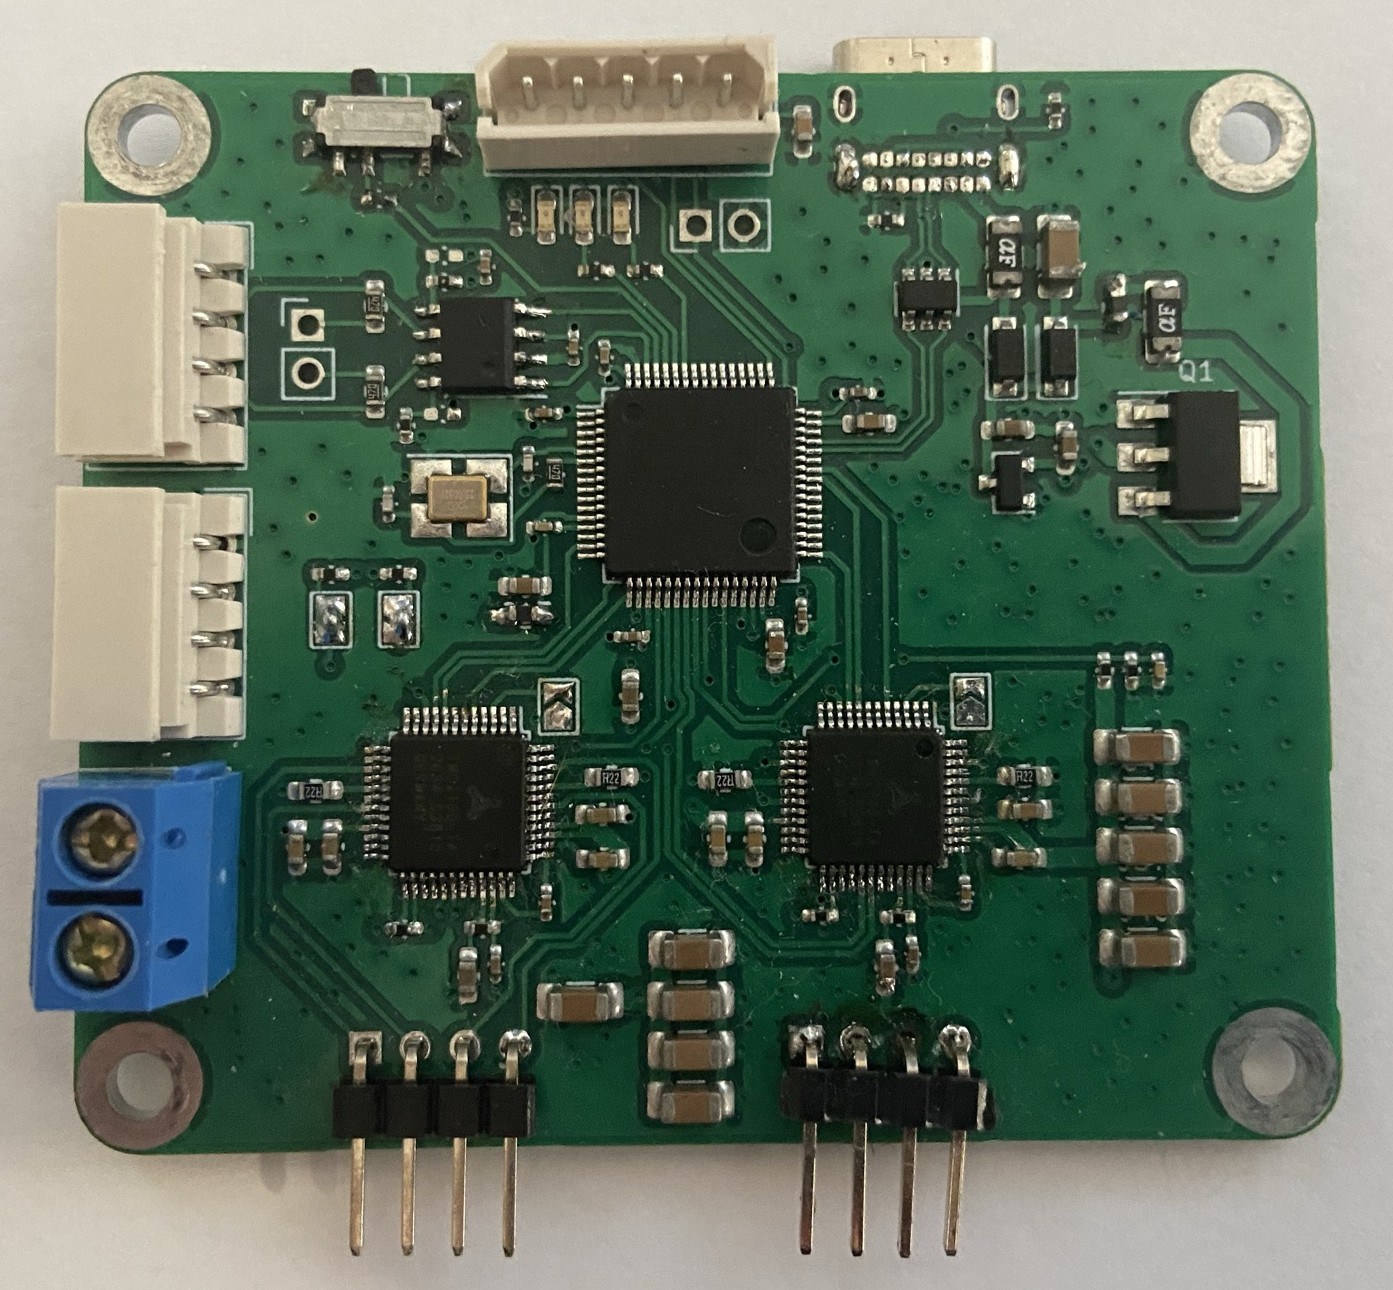
\includegraphics[height=0.9\textwidth]{obrazky/rev1}
        \caption{The manufactured revision 1 PCB.}
        \label{fig:rev1_pcb}
    \end{minipage}\hfill
    \begin{minipage}[t]{0.45\textwidth}
        \centering
        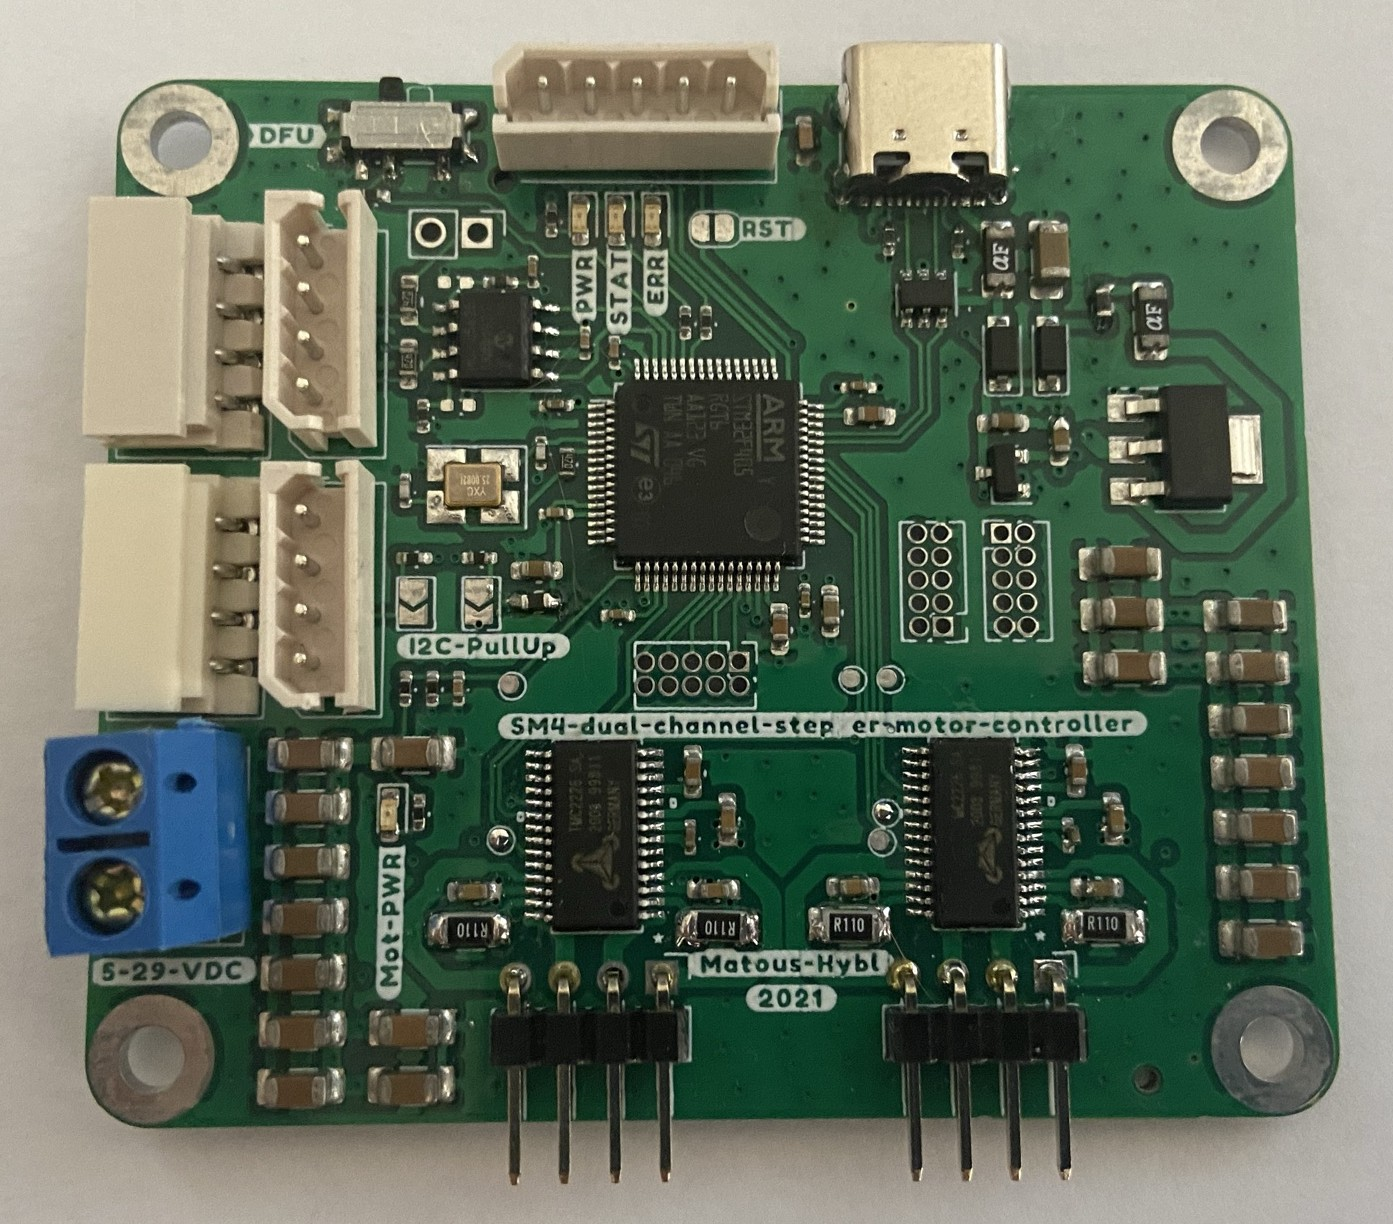
\includegraphics[height=0.9\textwidth]{obrazky/rev2}
        \caption{The manufactured revision 2 PCB.}
        \label{fig:rev2_pcb}
    \end{minipage}
\end{figure}

In general, two revisions of the hardware have been developed, but only the first one has been used for firmware development, due to time constraints.
Majority of the requirements have been fulfilled.
The stepper motor controller is capble of independently driving two stepper motors in either velocity or position mode.
Thanks to the Trinamic driver \acs{ic}s the motor operation is silent.
The driver now utilizes simulated encoders to measure output shaft position.
Given the controller's design, it can be controlled using the CANOpen protocol or via I\textsuperscript{2}C and can be configured using the USB interface.

\subsection{Requirements Fulfilment}
\label{subsec:req_fulfilment}
In the beginning of the development, we specified requirements in the Section~\ref{sec:requirements}.
Majority of the requirements have been fulfilled, but we will describe the unfulfilled requirements alongside their current fulfilment status in the Table~\ref{tab:unfulfilled_req}.

\begin{table}[H]
    \centering
    \begin{tabular}{ |p{2cm}|p{6cm}|p{6cm}| }
        \hline
        ID & Requirement & Fulfilment status \\
        \hline
        \hline
        FR-02 & When multiple communication interfaces are connected, the system shall prioritize CAN bus, then I2C. USB has the lowest priority. & We haven't been able to find a mechanism for prioritizing, we believe that this requirement might be changed as it should be the integrator's responsibility to choose only one of the communication interfaces. \\
        \hline
        FR-04 & All relevant values (currents, timings, limits, etc.) shall be configurable via USB or CANOpen SDO protocol. & Now, only a subset of the values is configurable, more values (such as configuration of communication) will be implemented in the future revisions. \\
        \hline
        NFR-03 & The controller shall be configurable using a program for personal computers. & The software for personal computers was developed, but the configuration part is missing as of now. \\
        \hline
        NFR-6 & The firmware should utilize software in the loop integration testing for \acs{qa} (\acl{Quality Assurance}) & Some software in the loop testing has been drafted with the Encoder abstraction, but more of the software in the loop testing will be done in the future.\\
        \hline
        NFR-7 & The firmware shall be properly documented. & Some parts of the firmware are already documented via the inline documentation, but the majority of the other code is not, but it will be done in the future revision. \\
        \hline
    \end{tabular}
    \caption{Unfulfilled requirements}
    \label{tab:unfulfilled_req}
\end{table}

\subsection{CANOpen API}
As we described in the Sections on firmware development (\ref{sec:firmware}) and the one on CANOpen (~\ref{subsec:canopen}), the firmware utilizes the Object Dictionary as the central configuration storage.
From the higher level systems, this Object Dictionary can be accessed via the SDO protocol using indexes and subindexes, that are specified in the Table~\ref{tab:object_dictionary} in the Appendix~\ref{ch:canopen_appendices}.

Apart from accessing the Object Dictionary using SDOs, some of the important control and configuration values have been made accessible via the PDO protocol.
The structure of the PDOs can be seen in the Tables~\ref{tab:rxpdo1}, \ref{tab:txpdo1}, \ref{tab:velocity_pdo}, \ref{tab:position_pdo} in the Appendix~\ref{ch:canopen_appendices}.
For completeness, the description of the PDOs can be found in the Table~\ref{tab:pdo_meaning}.

\begin{table}[H]
    \centering
    \begin{tabular}{ |p{3cm}|p{10cm}| }
        \hline
        Name & Contents \\
        \hline
        \hline
        TxPDO1 & Contains device status - battery voltage and temperature \\
        \hline
        TxPDO2 & Contains actual velocities of both axes \\
        \hline
        TxPDO3 & Contains actual position of axis 1 \\
        \hline
        TxPDO4 & Contains actual position of axis 2 \\
        \hline
        RxPDO1 & Sets axis mode and enables axes \\
        \hline
        RxPDO2 & Sets target velocities for both axes \\
        \hline
        RxPDO3 & Sets target position for axis 1 \\
        \hline
        RxPDO4 & Sets target position for axis 2 \\
        \hline
    \end{tabular}
    \caption{Simplified PDO contents}
    \label{tab:pdo_meaning}
\end{table}

Alongside the SDO and PDO protocols, also the SYNC and NMT protocols have been implemented.
Note that the device must reach the NMT State Operational in order to enable motion control.

\subsection{I\textsuperscript{2}C API}
In order for the controller to be usable with the BPC-PRP course, we developed a simplified API for the I\textsuperscript{2}C bus.
Using this API, it is only possible to set the axes mode, enable or disable them and then to set control variables and read them.
In the course, the students utilize control in the velocity mode and then acquire the positions of both axes for odometry calculation.
In the previous Sections, we described that in order for motion control to work, the driver needs to reach NMT State Operational.
With the I\textsuperscript{2}C API, this transition is performed automatically when the axes are enabled.

The API can be found in the Table~\ref{tab:i2c_api} and is based on the I\textsuperscript{2}C protocol described in the Figures~\ref{fig:i2c_r} and \ref{fig:i2c_w}.

\begin{table}[H]
    \centering
    \begin{tabular}{ |p{3cm}|p{2cm}|p{2cm}|p{6cm}| }
        \hline
        Address & R/W & Length [B] & Description \\
        \hline
        \hline
        0x10 & R/W & 2 & axis mode and axis enable \\
        \hline
        0x2X & R/W & 4 & set or read axis velocity, where X denotes the axis (1, 2) \\
        \hline
        0x3X & R/W & 8 & set or read axis position, where X denotes the axis (1, 2) \\
        \hline
        0x40 & W & 8 & set velocity for both axes \\
        \hline
        0x50 & R & 16 & read position from both axes \\
        \hline
    \end{tabular}
    \caption{I\textsuperscript{2}C API}
    \label{tab:i2c_api}
\end{table}

\subsection{USB API}
The implemented USB API was designed to only allow for configuring the device as per the requirements.
The protocol is fairly simple, there are two types of messages - a request and a transfer message, that can be seen in the Figures~\ref{fig:usb_request} and \ref{fig:usb_tansfer}.

When the higher level device wants to write a value to the Object Dictionary, it simply sends the data transfer message, where the OD KEY contains the index and the subindex.
On the other hand, when the higher level device wants to read a value from the Object Dictionary, it sends the data request message and the controller responds with the data transfer message containing the requested value.

\begin{figure}[H]
    \centering
    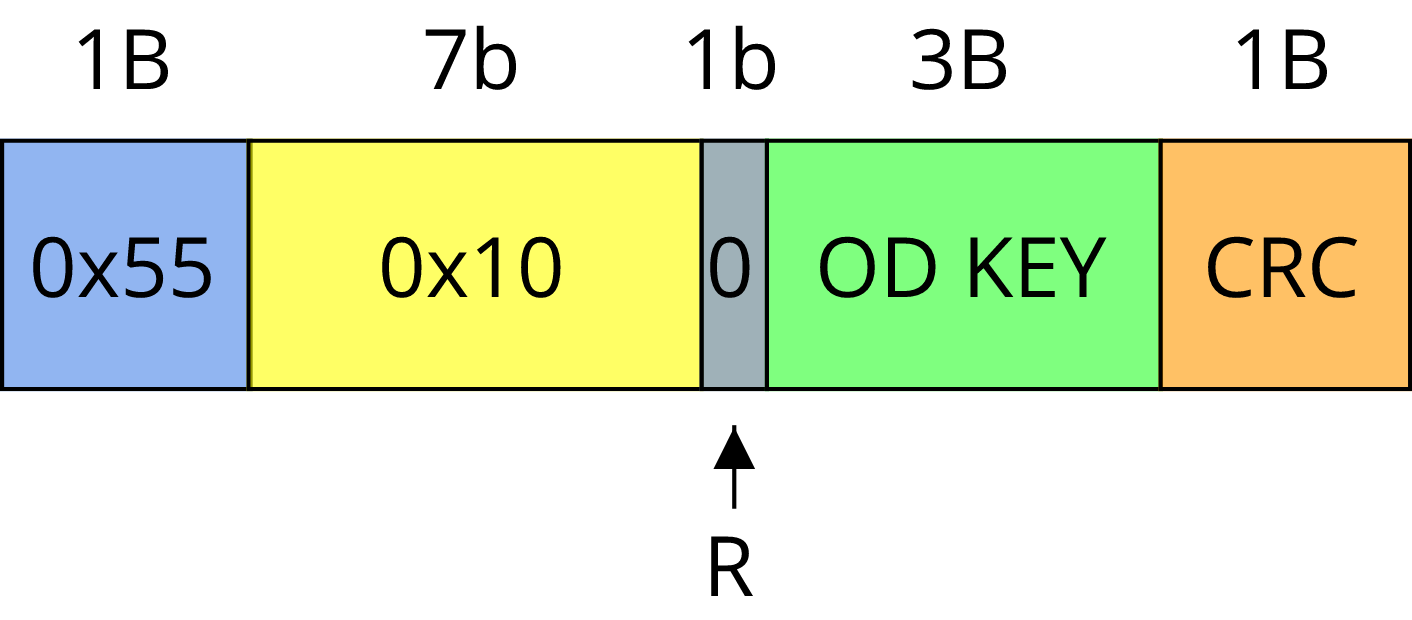
\includegraphics[width=0.4\textwidth]{obrazky/usb_request}
    \caption{A data request in the USB API.}
    \label{fig:usb_request}
\end{figure}

\begin{figure}[H]
    \centering
    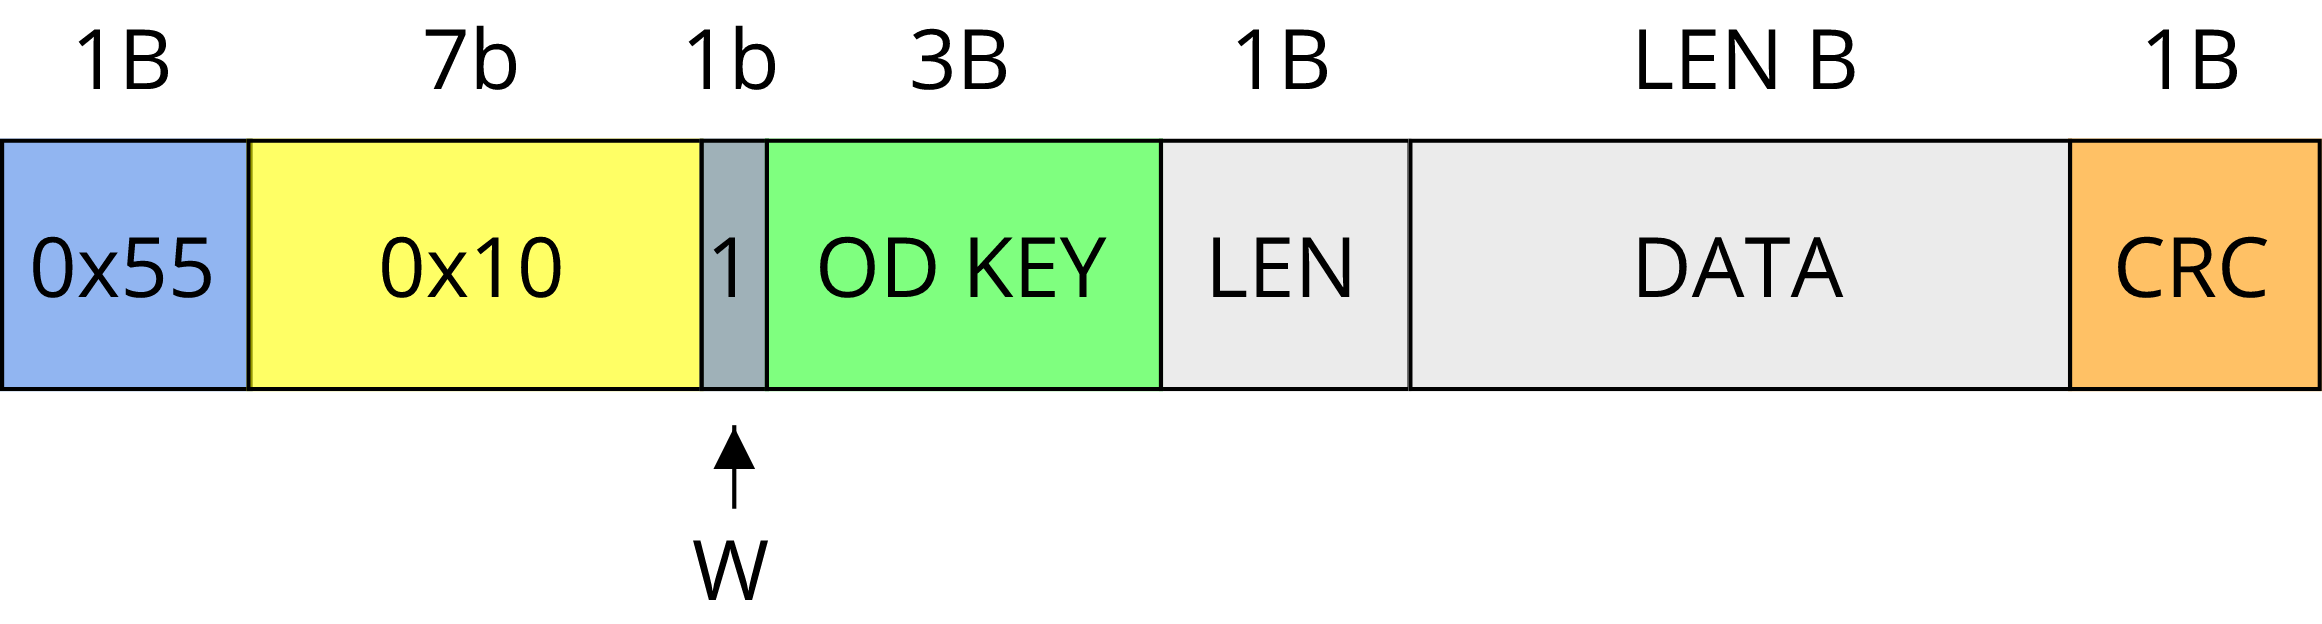
\includegraphics[width=0.7\textwidth]{obrazky/usb_transfer}
    \caption{A data transfer in the USB API.}
    \label{fig:usb_tansfer}
\end{figure}

\subsection{Communication Failure Failsafe}
A simple failsafe for the cases when the communication stops was employed.
The failsafe triggers when no control message is received for a specific amount of time.
Therefore it is vital to send the control data periodically.
This is true for both the CANOpen and I\textsuperscript{2}C APIs.


\subsection{Control Application}
A simple control application utilizing the \acs{tui} and CANOpen protocol was developed.
Controlling the stepper motor controller both in velocity and position mode is implemented, but it is not possible to change controller parameters, such as controller constants.
In the future a fully featured control application with proper \acs{gui}, support for all the buses and configuration will be developed in order to allow for seamless configuration.
Adding support for flashing via \acs{usb} \acs{dfu} is planned too.

\subsection{Takeaways for Future Revisions}
\label{subsec:final_takeaways}
In this section, we describe what changes we'd made in a possible future revisions.
The changes are:
\begin{itemize}
    \item Use the angular XT-30 connector for motor power.
    \item Use different connectors for motors.
    \item Use standardized 10 pin JTAG connector for SWD (Serial Wire Debug).
    \item Use eFuse for electronics protection.
    \item Add more status LEDs.
    \item Improve encoder connector placement, select appropriate connectors.
    \item Remove compatibility resistors around the CAN transceiver.
    \item Attempt to utilize async Rust for easier development.
    \item Rework the schematic to include more information, such as maximal capacitor voltages, add reasoning about component values.
    \item Improve current sensing circuitry to support motors with different phase currents and use sensing resistors with proper power rating. The current should be easily configurable.
    \item Use 4 byte key for object dictionary values.
    \item Properly configure bxCAN filters for CANOpen operation.
\end{itemize}

\section{Demonstration \#1 - Linear Rail Actuator for Camera Movement}
\label{sec:dem2}
The first demonstration for the SM4 motor controller is controlling a single axis linear rail actuator.
This actuator was provided by the thesis supervisor and is equipped with a NEMA17 style stepper motor that drives a belt with an attached table.
Originally, this rail was meant to be used for camera movement when recording a musician.

This demonstration is controlled using a Raspberry Pi 4B, and the SM4 motor controller is controlled using the I\textsuperscript{2}C bus and the corresponding API.
This showcase aims to demonstrate the controller's ability to control in position mode and therefore to position the table on the rail according to the commands of the higher-level system, and also the usability of I\textsuperscript{2}C bus and API.
In the future, this demonstration will be equipped with a second axis allowing for tilting the mounted camera.
The finished demonstrator can be seen in the Figure~\ref{fig:rail_demonstrator}.

\begin{figure}[H]
    \centering
    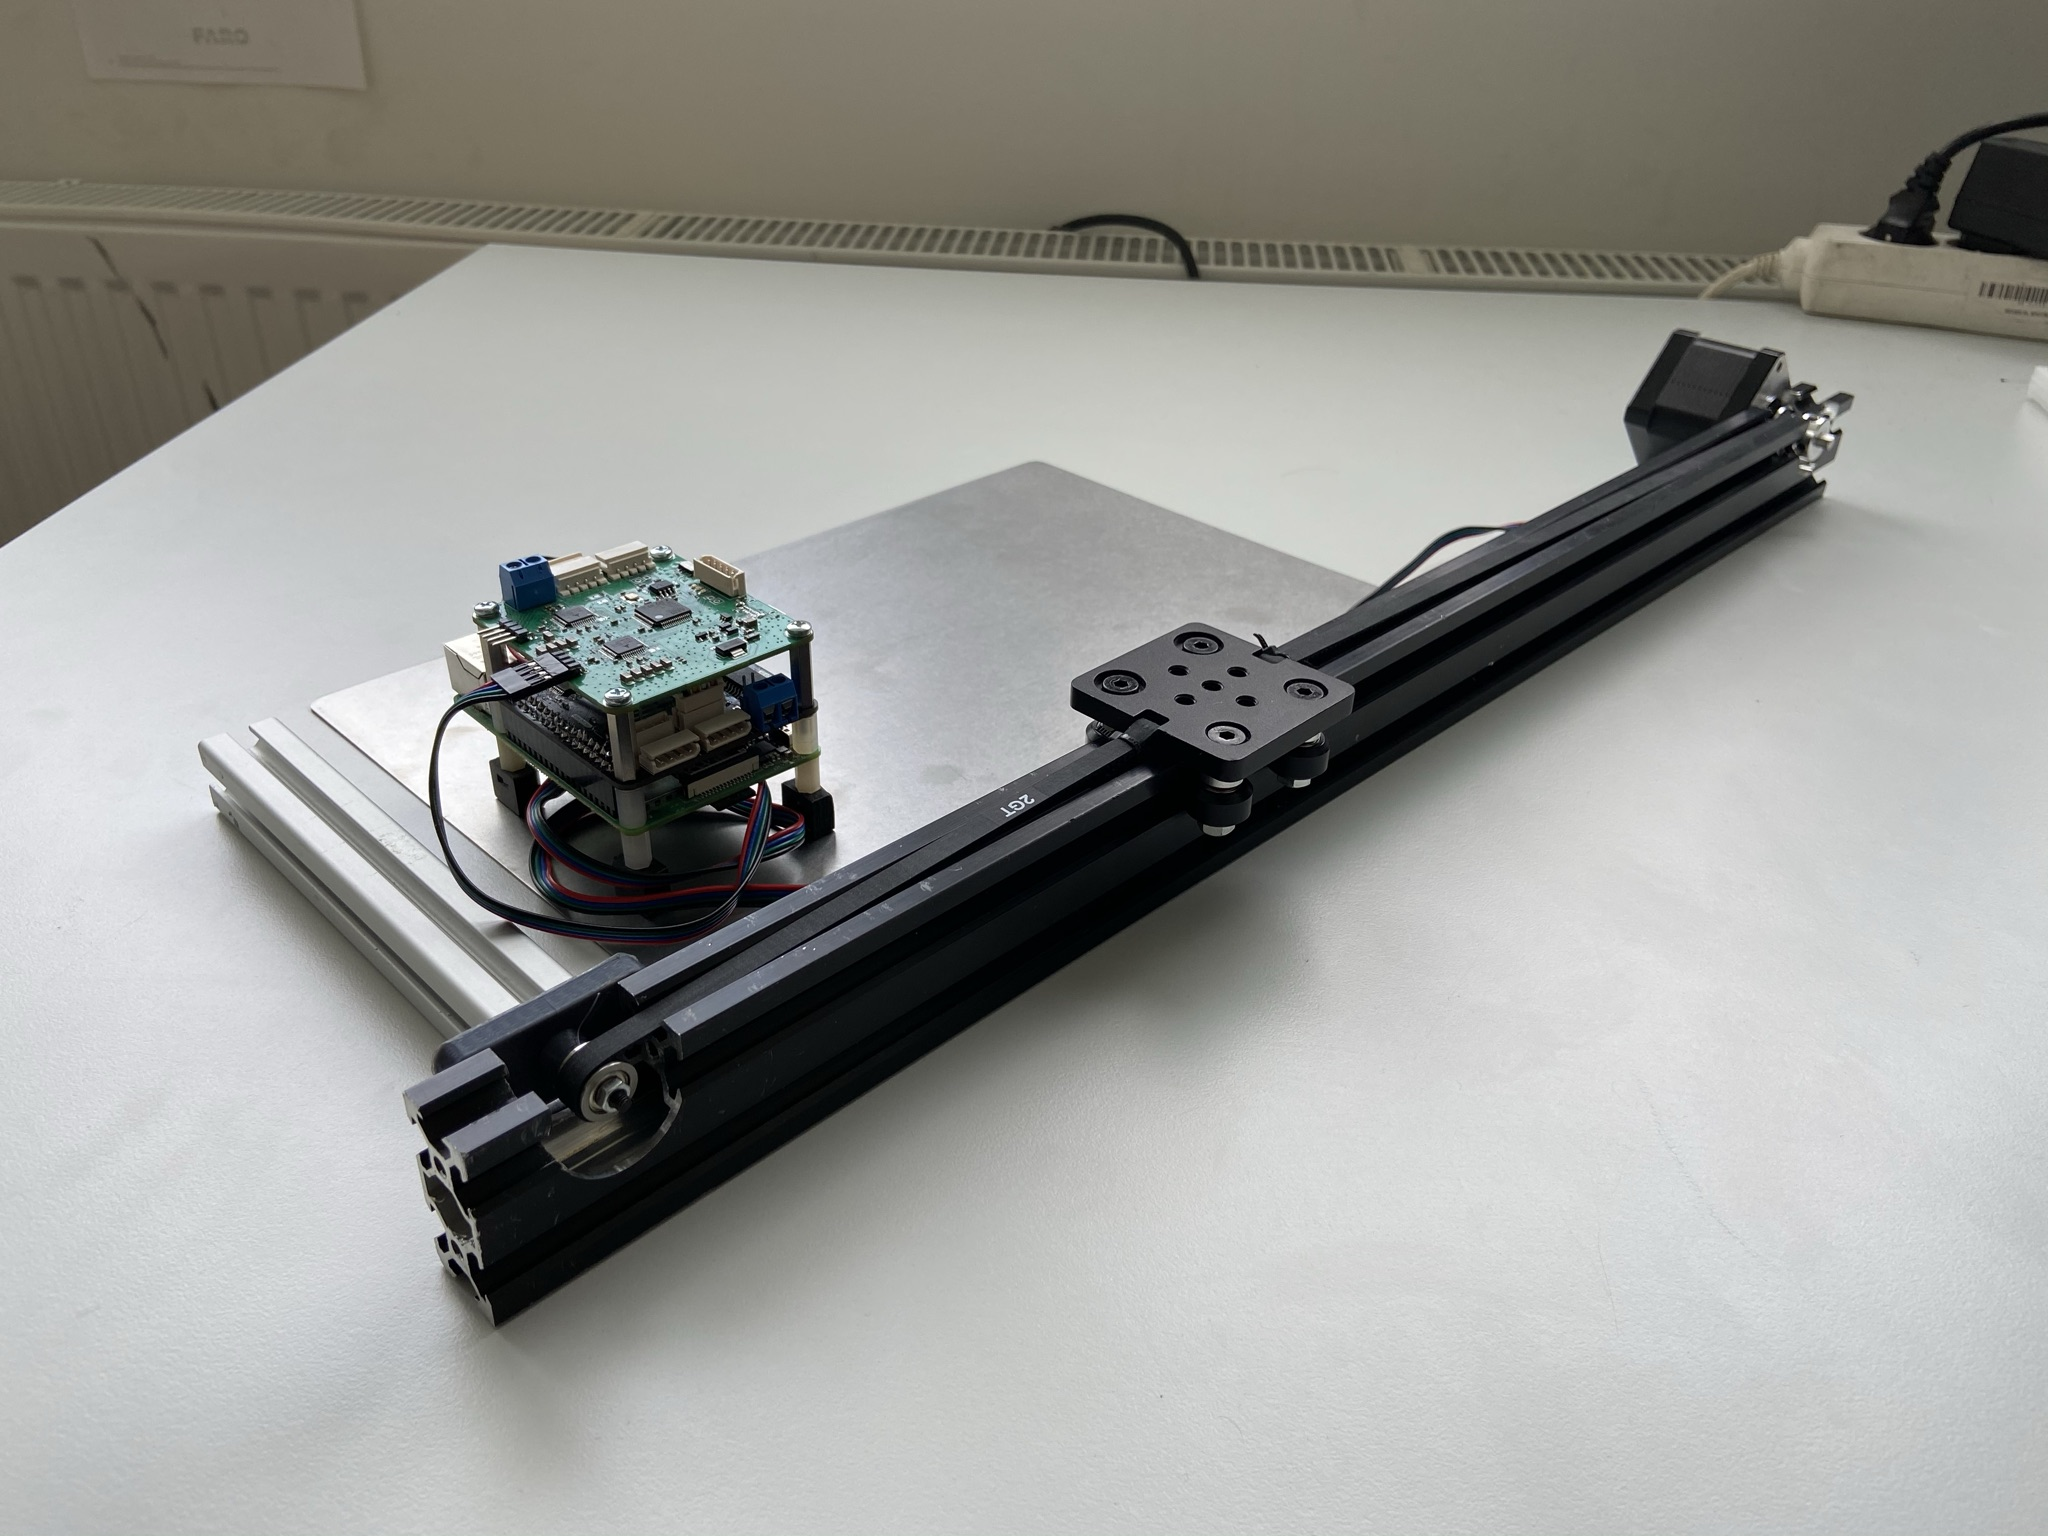
\includegraphics[width=0.7\textwidth]{obrazky/rail}
    \caption{The MAP-bot robot - the first demonstration of the SM4 stepper motor controller.}
    \label{fig:rail_demonstrator}
\end{figure}

\section{Demonstration \#2 - Small Mobile Robot for Indoor Mapping}
\label{sec:dem1}
\epigraph{
    Any exploration program which "just happens" to include a new launch vehicle is, de facto, a launch vehicle program. \newline\newline
    (alternate formulation) The three keys to keeping a new human space program affordable and on schedule: \newline
1)  No new launch vehicles. \newline
2)  No new launch vehicles. \newline
3)  Whatever you do, don't develop any new launch vehicles.}{Akin's Laws of Spacecraft Design\cite{akin_akins_nodate}}

The second demonstration, where we showcase the SM4 stepper motor controller, is a small differentially driven robot aimed for indoor mapping and self-localization.
The chassis is differential with a motor on two sides of the robot, which showcases the driver's ability to control both of the motor and calculate odometry.
Apart from the driver itself, the robot features a Raspberry Pi 4B SBC, 4 cell Li-Ion battery, step-down converter and a simple planar LIDAR for the mapping task.
A block diagram of this demonstration can be seen in the Figure~\ref{fig:mapbot_block}

\begin{figure}[H]
    \centering
    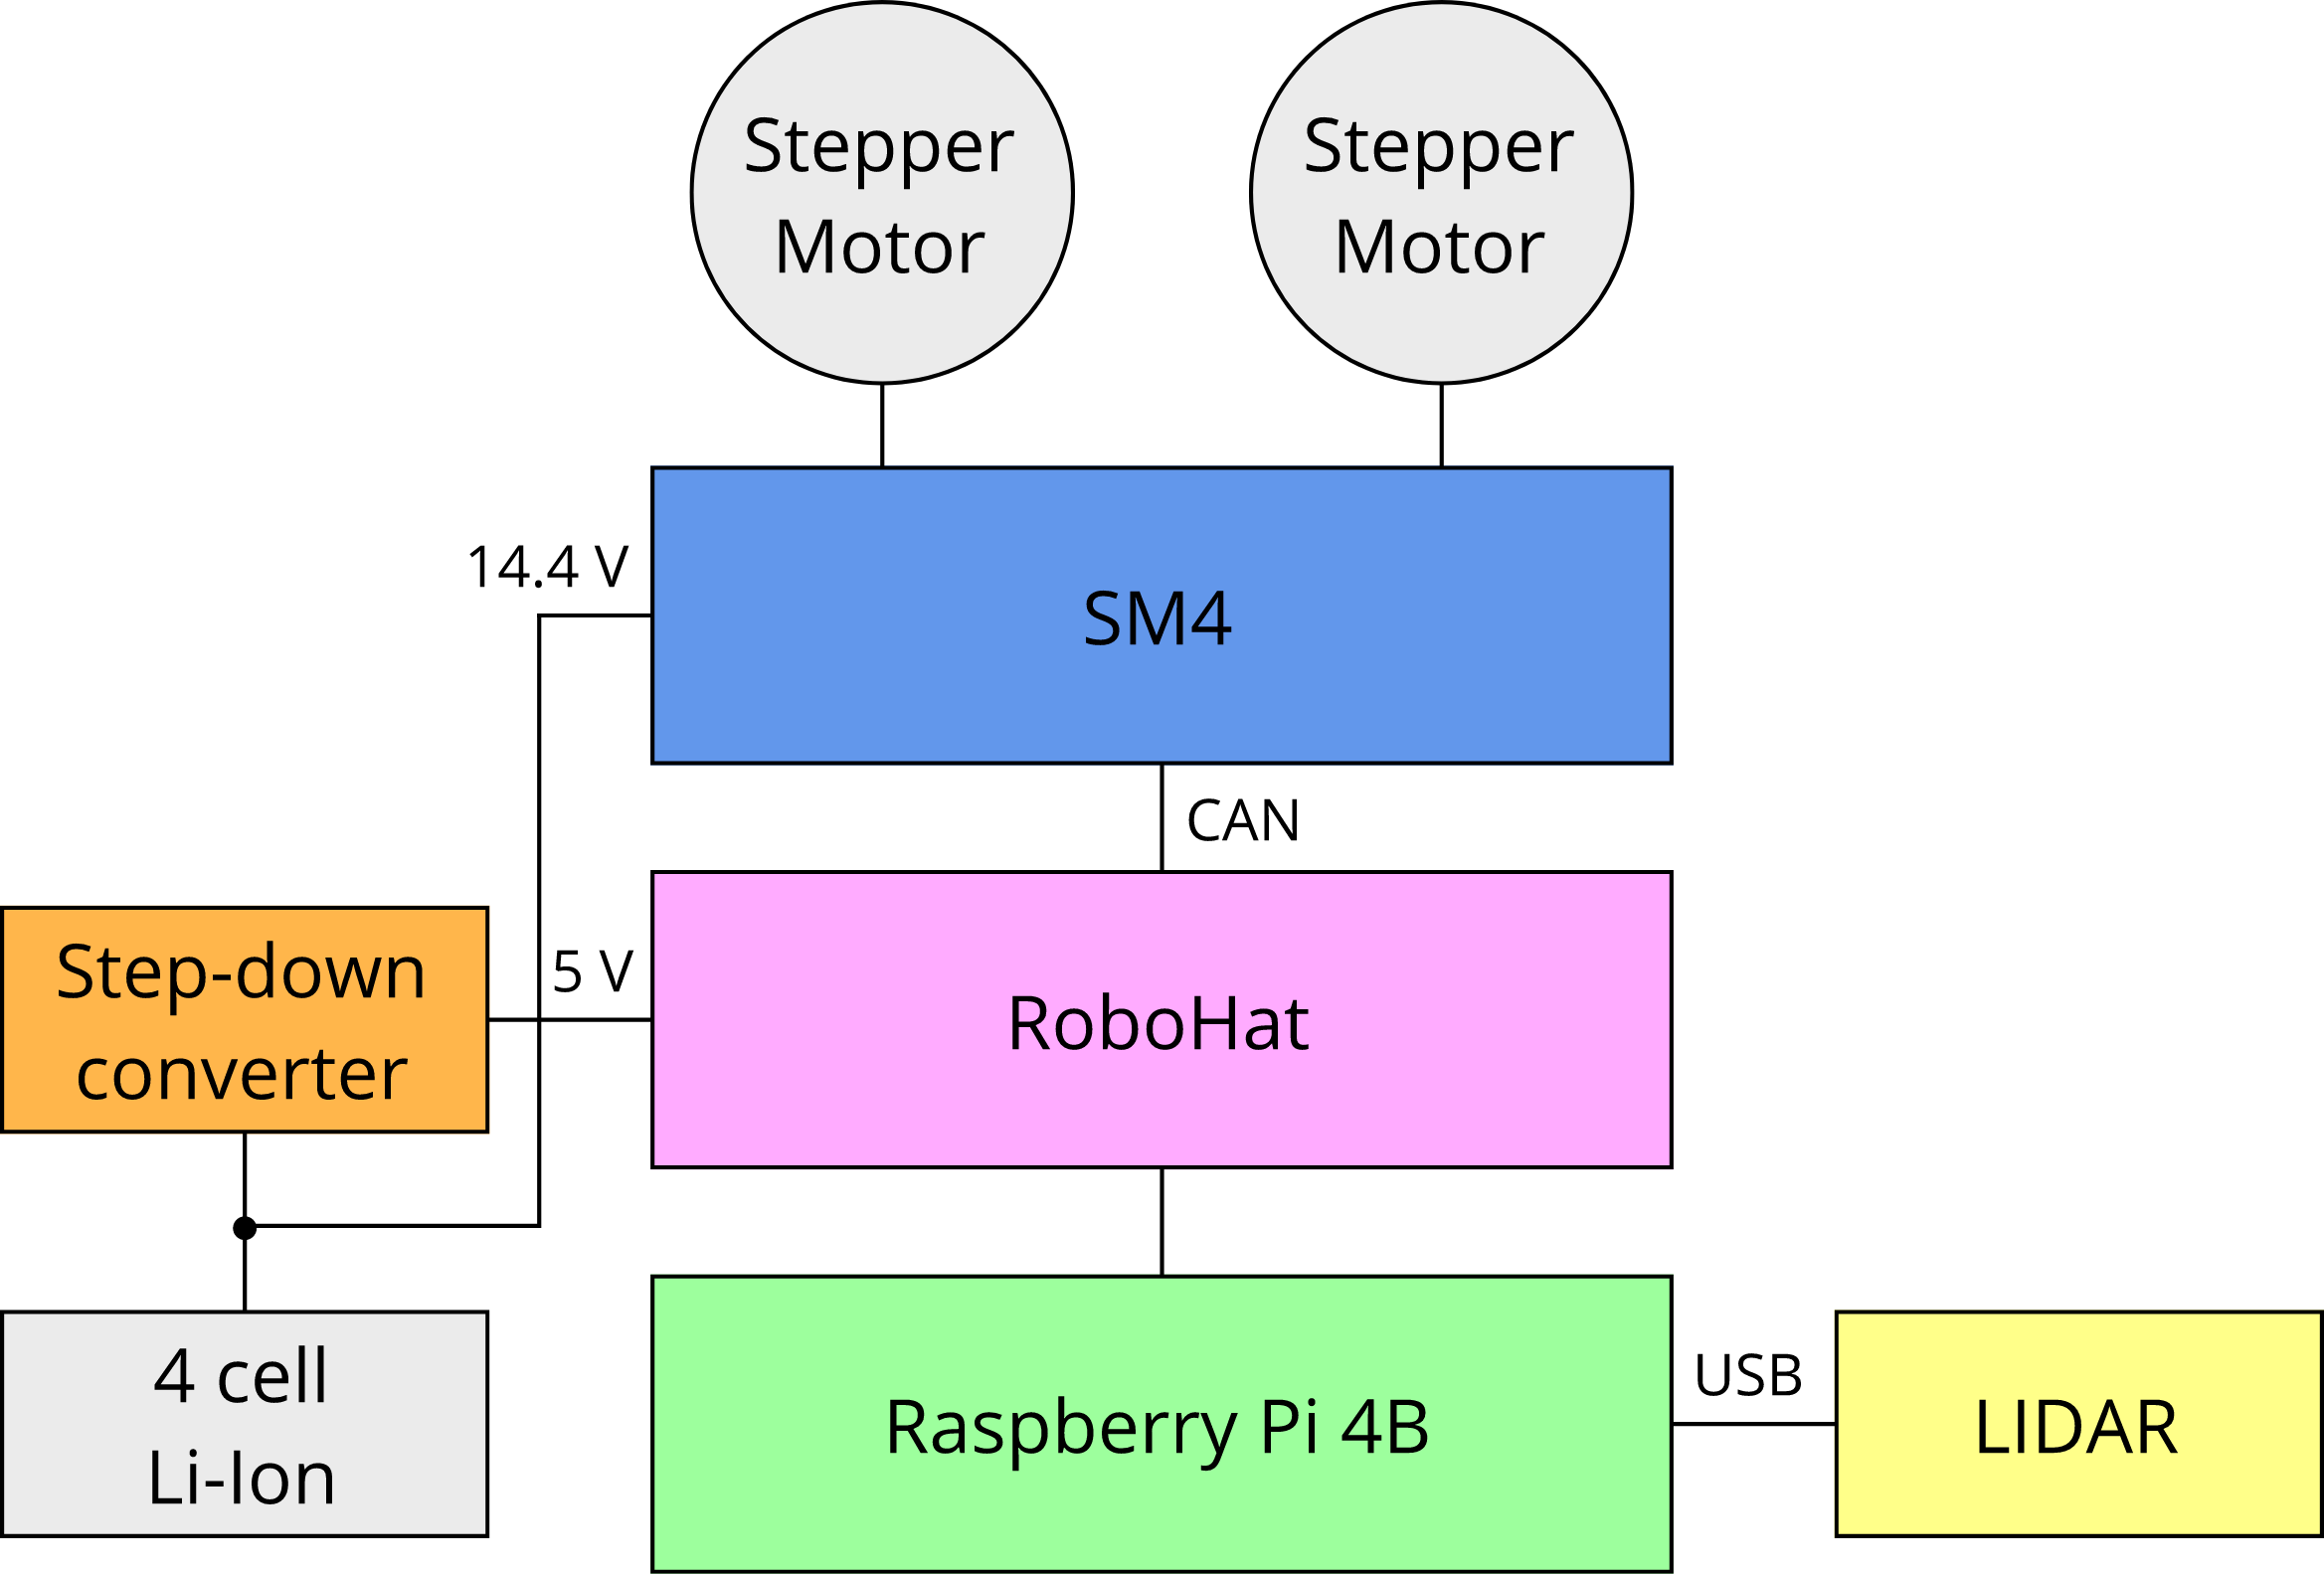
\includegraphics[width=0.9\textwidth]{obrazky/mapbot_block_diag}
    \caption{The block diagram of the robot used for the second demonstration.}
    \label{fig:mapbot_block}
\end{figure}

It is projected, that the robot will be utilized for algorithm demonstration as part of the MPC-MAP - Advanced Mapping and Self-Localization for Robotics course.
The finalized robot can be seen in the Figure~\ref{fig:map_bot}.

\begin{figure}[H]
    \centering
    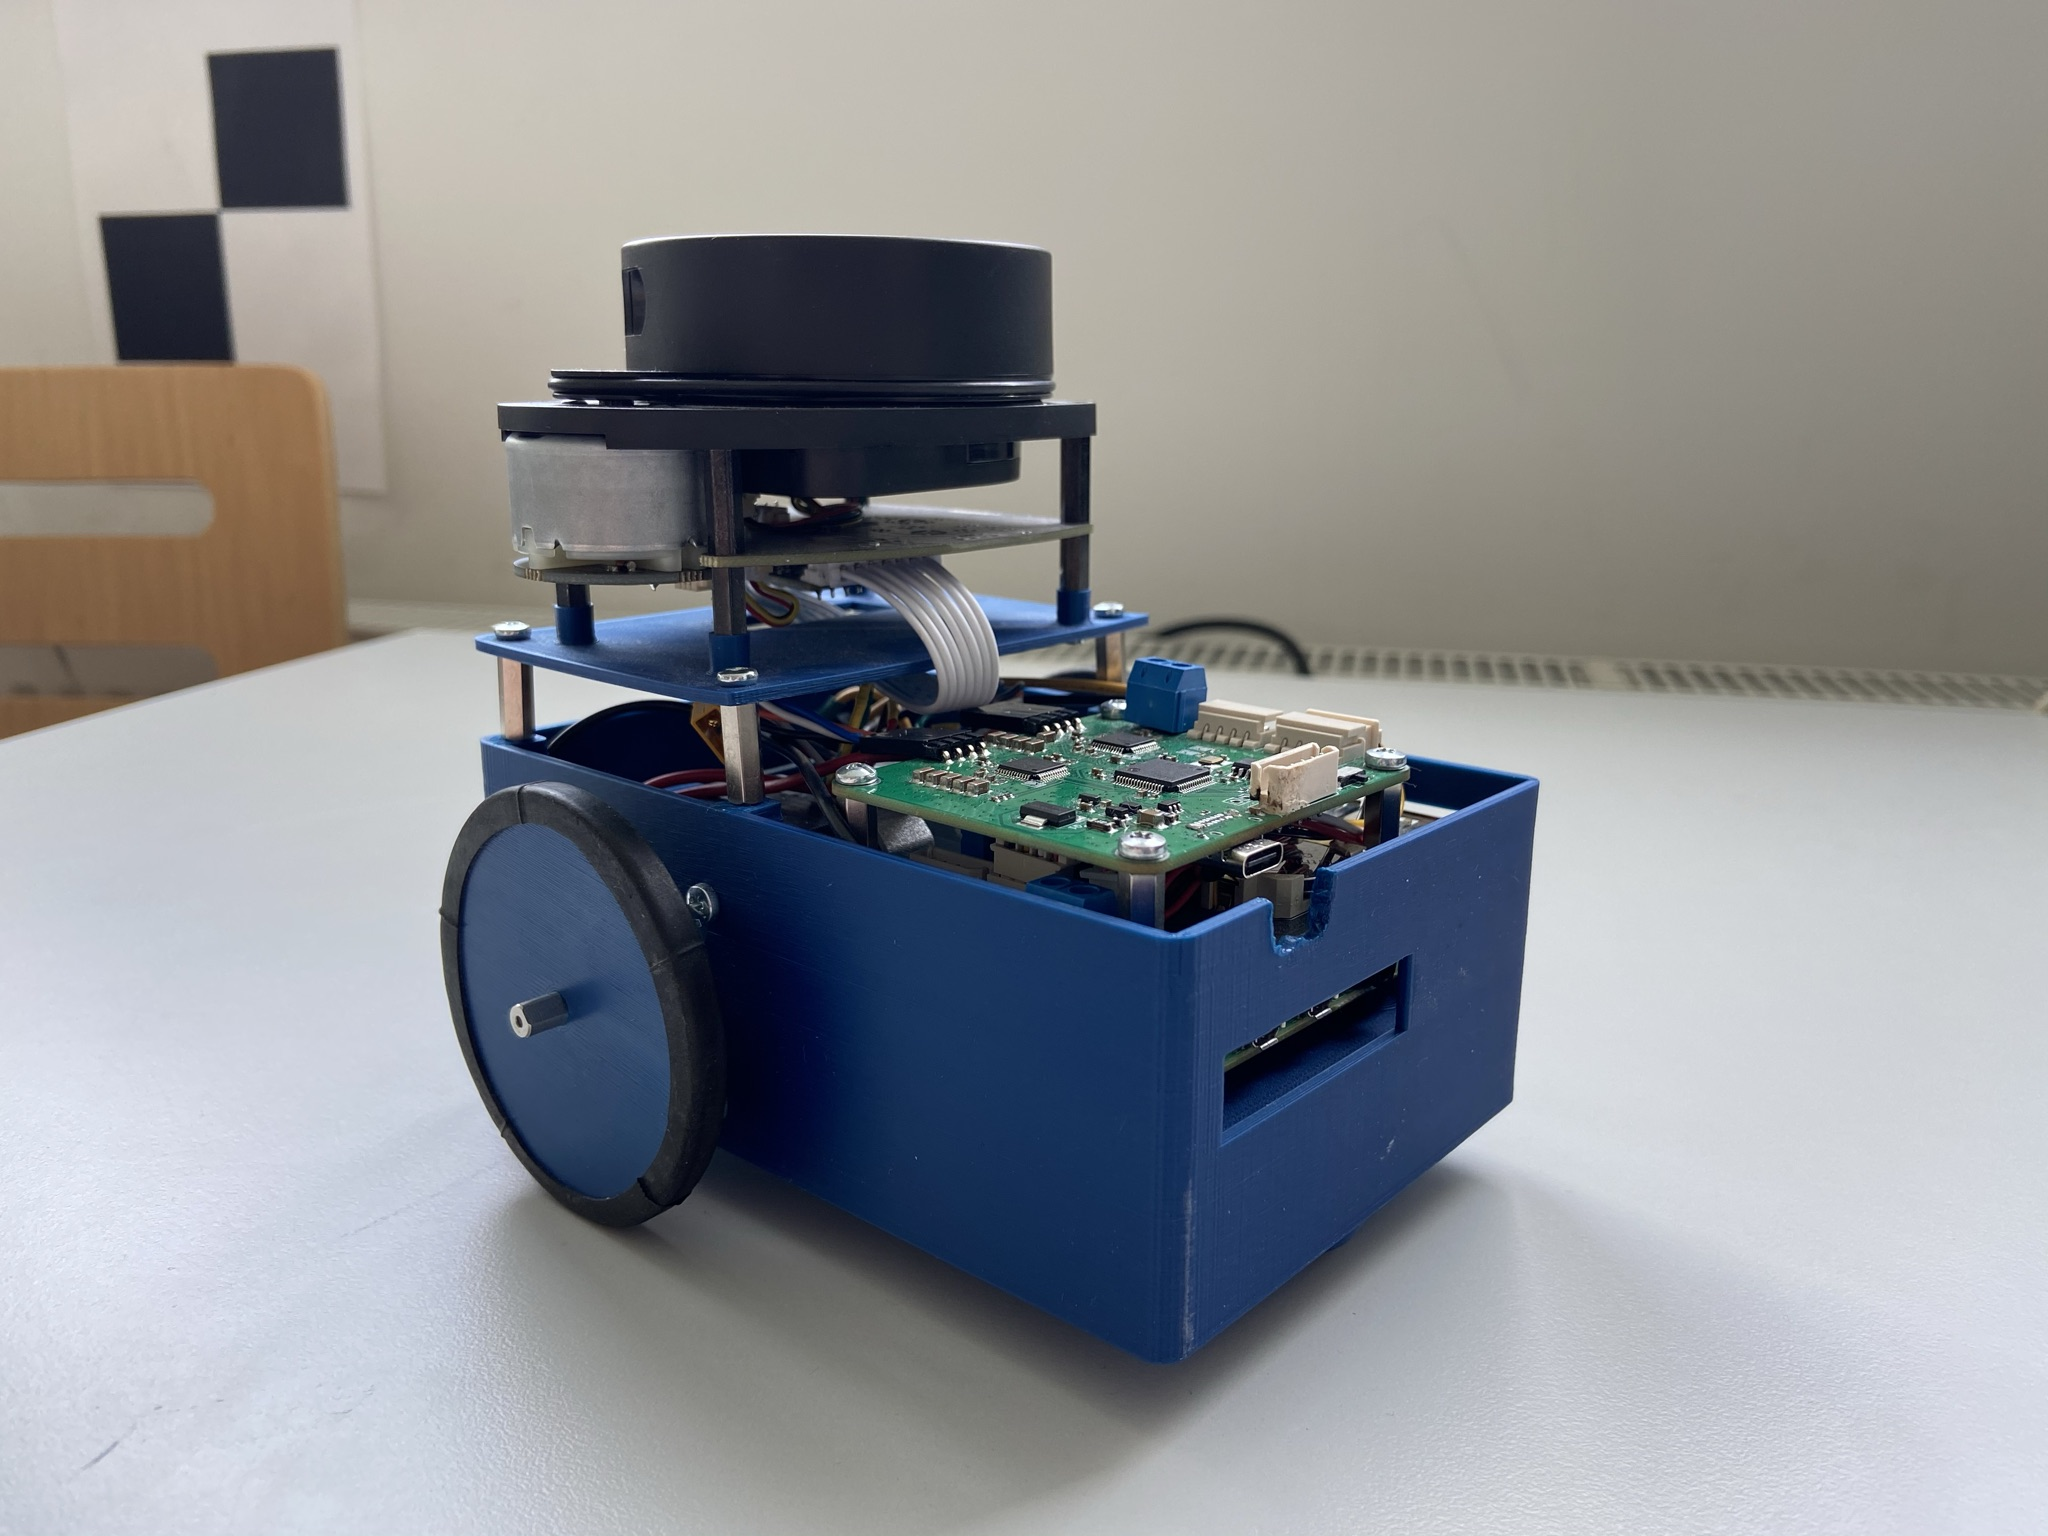
\includegraphics[width=0.7\textwidth]{obrazky/map_bot}
    \caption{The MAP-bot robot - the first demonstration of the SM4 stepper motor controller.}
    \label{fig:map_bot}
\end{figure}
